\section{DBToaster Overview}

\noindent\textbf{Data and Query Model.}
\compiler\ focuses on applications issuing standing queries on a database which
subsequently process continuously changing, large volumes of input tuples.
\compiler\ is capable of compiling a wide variety of SQL queries including the
core relational algebra, standard aggregates (\texttt{sum}, \texttt{avg},
\texttt{count}, \texttt{min}, \texttt{max}), subqueries and nested aggregates.
Our data model differs from today's data stream processors, in that we consider a
database as a set of relations each subject to an arbitrary sequence of inserts,
updates and deletes. In contrast, data stream processors assume a well-defined
separation between tuples' insert and delete operations on the stream (value- or
count-based windows), or assume ordered deletion semantics (punctuations or
heartbeats). In \compiler, each tuple has an arbitrary lifetime, thus our
standing queries process a database spanning an arbitrary valid time using
temporal database terminology. Indeed, many stream applications, such as
order book trading and moving object applications, are self-managing, in that the
application logic and delta patterns ensure that state does not grow unboundedly in
practice.

\comment{
\begin{figure}[tb]
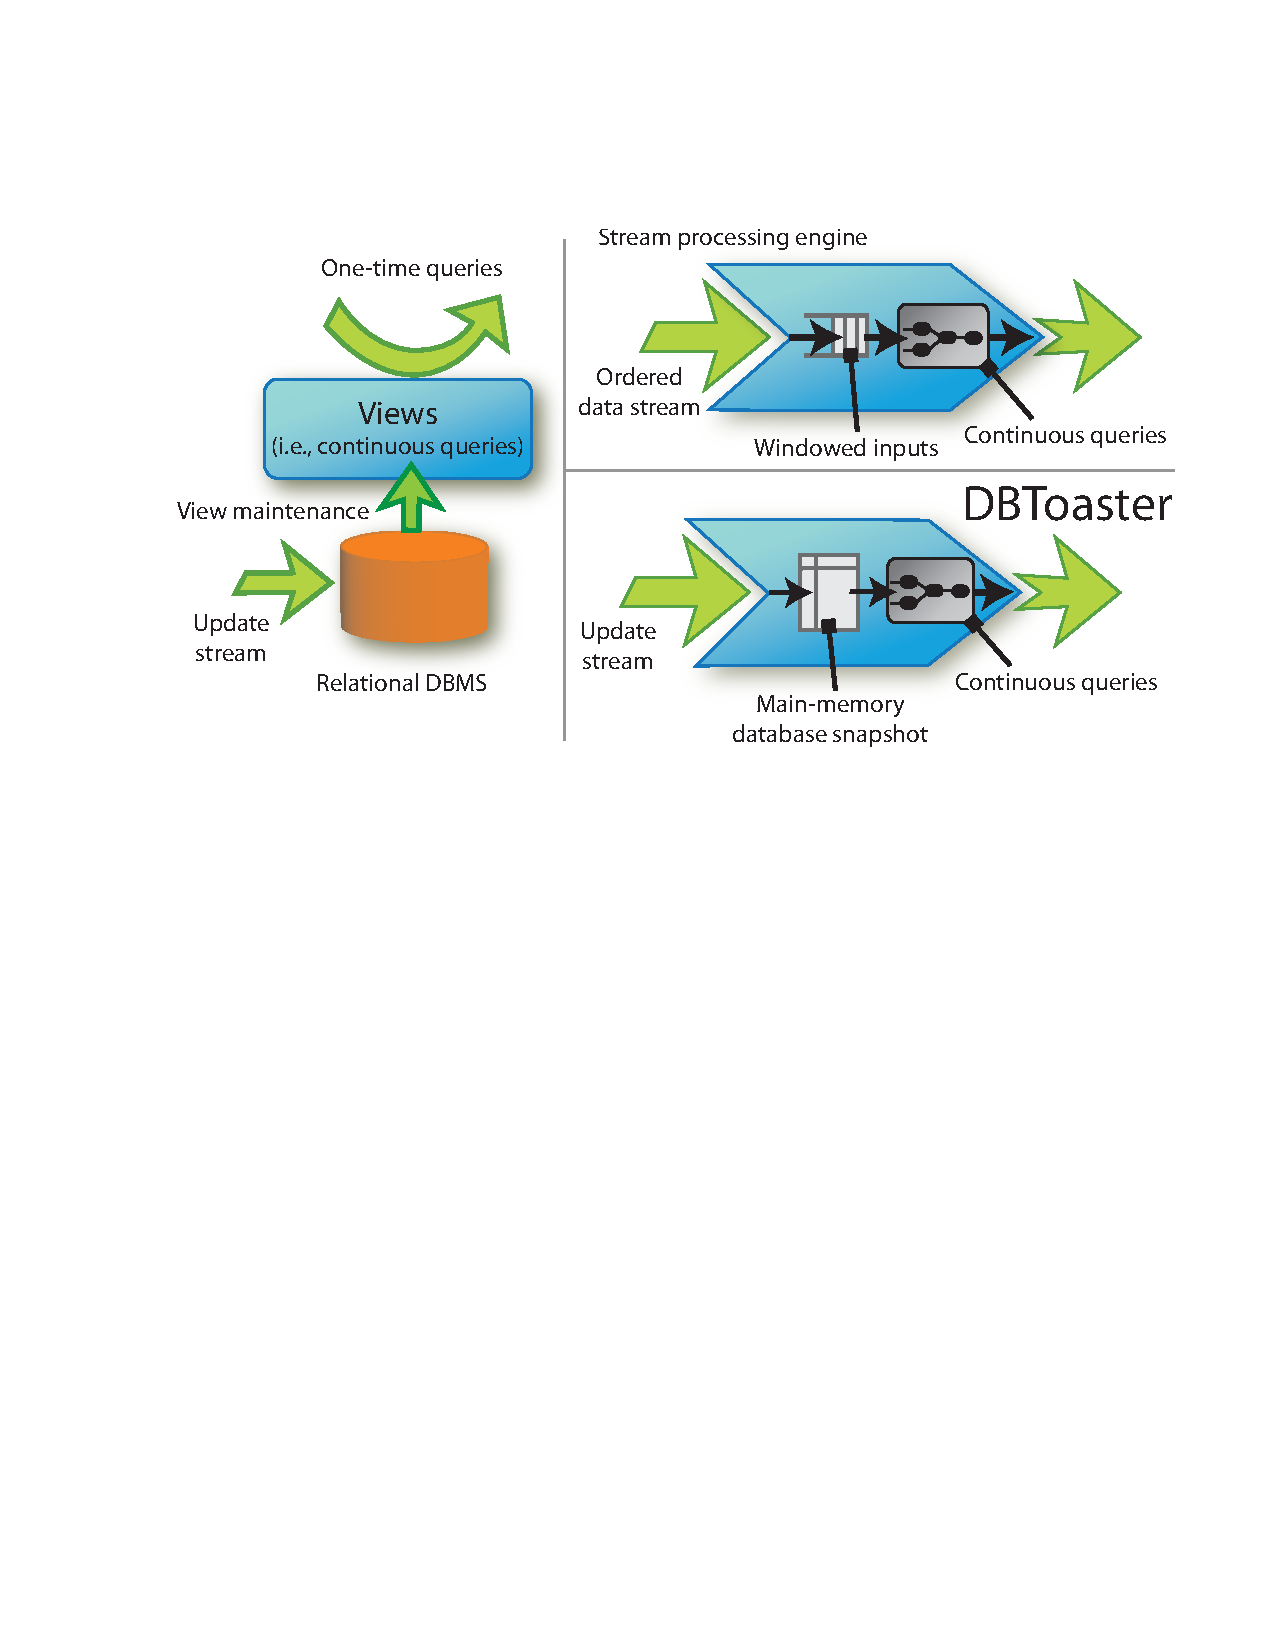
\includegraphics[scale=0.5]{figures/dbt-datamodel.pdf}
\label{fig:datamodel}
\caption{\compiler\ data model, in contrast to traditional DBMS and stream
processors.}
\end{figure}
}

\begin{figure}[tb]
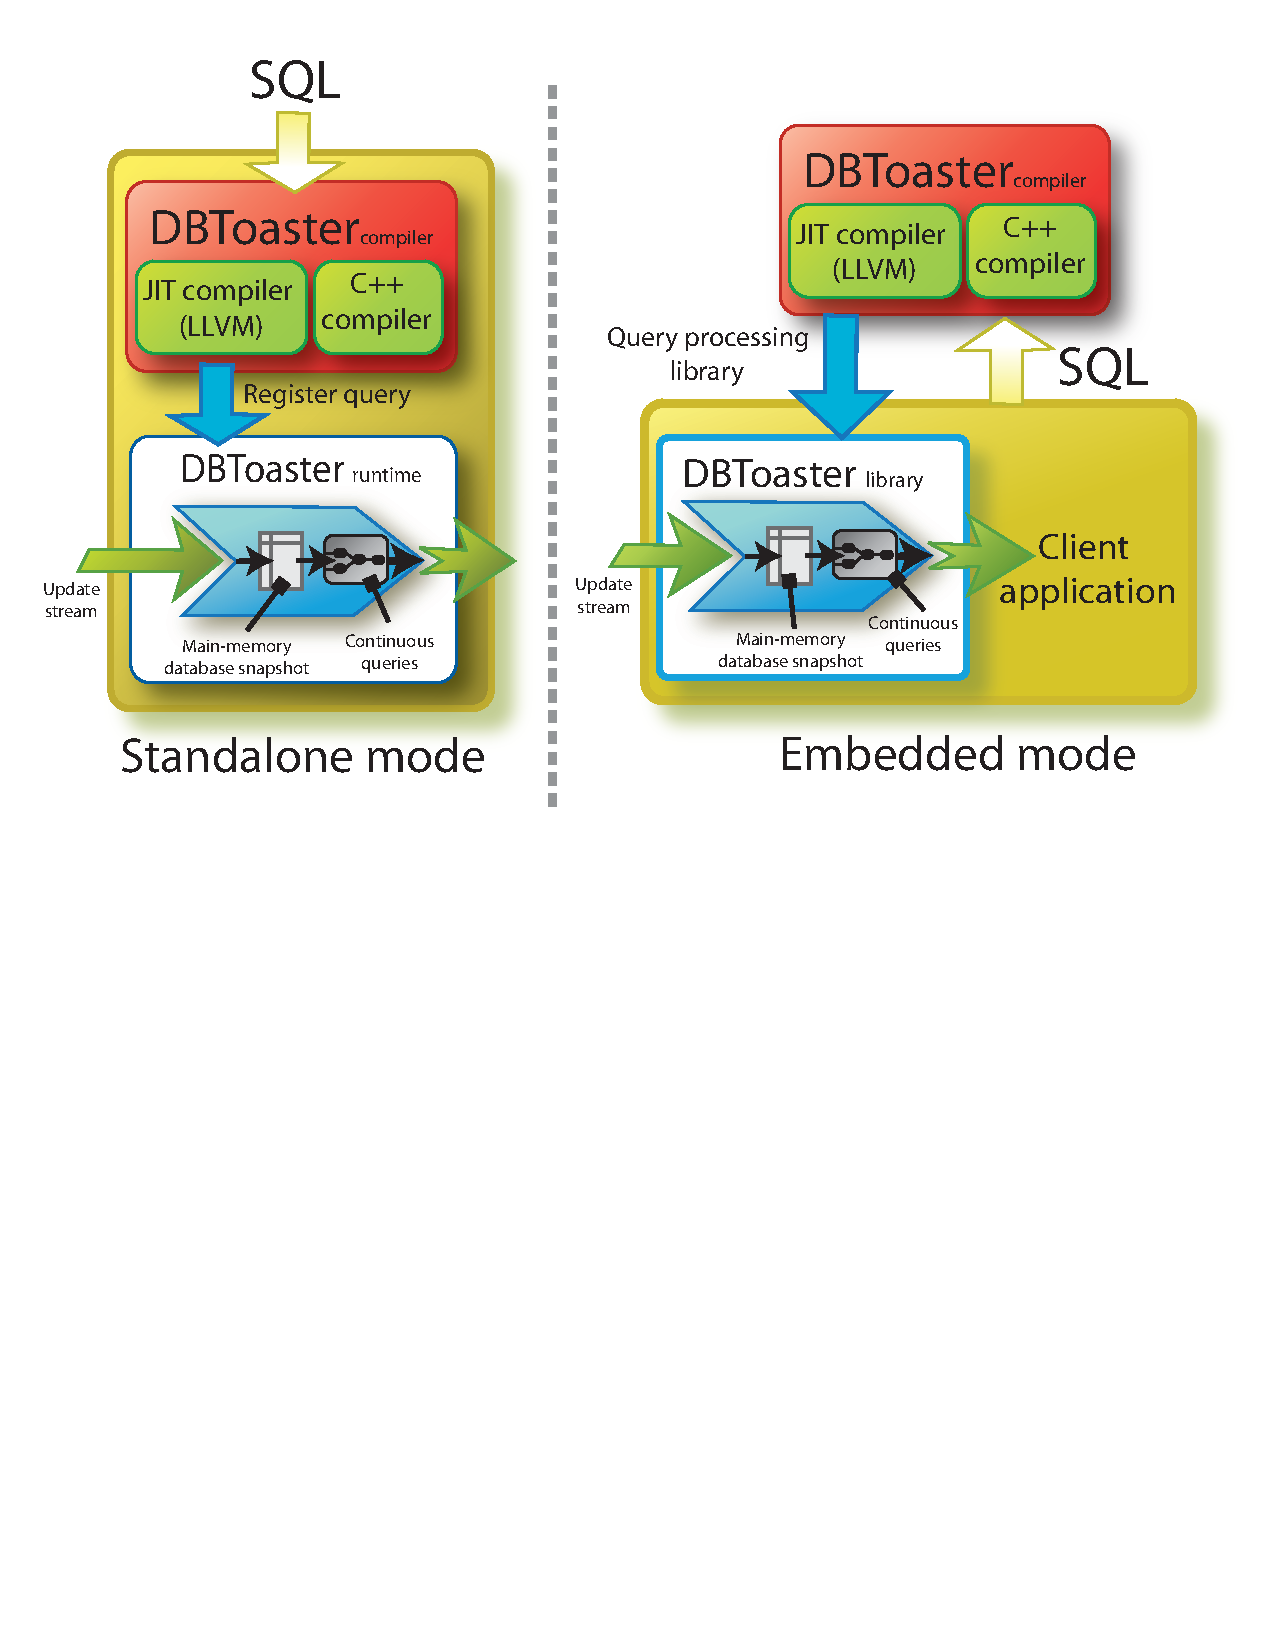
\includegraphics[scale=0.42]{figures/dbt-arch.pdf}
\label{fig:dbtarch}

\vspace{-6mm}

\caption{\compiler\ architecture, illustrating standalone and embedded modes of
query processing. In standalone mode, \compiler\ produces a lightweight
runtime, while in embedded mode, \compiler\ can alternatively produce a binary
library that can be used directly in client applications.}

\vspace{-4mm}

\end{figure}

\smallskip

\noindent\textbf{System Model.}
At its core, \compiler\ consists of a parser, an algebraic compiler and a code
generator. Our compilation workflow produces a delta-processing function for each
type of delta (insert, update or delete) on any base relation used in the query.
In addition, compilation defines in-memory aggregate views that are maintained
during runtime to support our delta-processing functions. We will see how these
data structures are defined in the description of our algorithm below. The
\compiler\ runtime may be used as a standalone query processor accepting input
over a network interface or archived stream, or as an embeddable query processor
that can be directly compiled into the same address space as application logic.
\compiler\ also exposes a read-only interface to its internal data structures to
support ad-hoc client-side queries. \compiler\ includes a debugger and profiler
for tracing delta processing functions and their maintenance of internal data
structures.

\comment{
\section{DBToaster Usage}

\compiler\ is capable of compiling a wide variety of SQL queries including those
containing selections, projections, joins, and group-by aggregates. \compiler\
takes a query workload as input, as well as the data definition statements of any
tables used in the queries to determine the contents of internal datastructures,
and produces a native binary for processing the query workload over inserts,
deletes and updates on the input tables. \compiler\ focuses on applications faced
with handling a large input volume, but does not rely on artificial restrictions
of these new inputs, unlike stream processing engines, which rely on semantic
constructs such as windows or punctuations that are tightly coupled with operator
semantics. Indeed, many stream applications, such as order book trading are
self-managing, in that the application logic and usage patterns ensures state
does not grow unbounded eliminating the need for windows. Otherwise, windows may
often be expressed as predicates. \compiler\ will compile such window semantics
just as with any other part of the query, and as we will see later, efficiently
implement windowing based on the data structures used to process the windowing
predicate.

\begin{figure}
\begin{center}
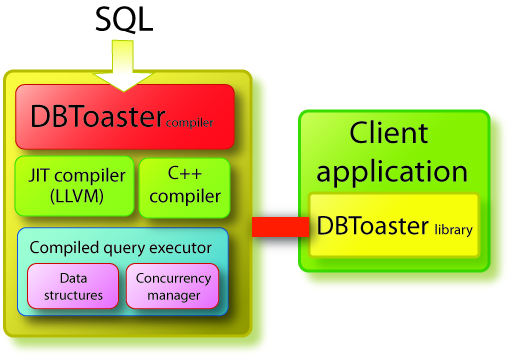
\includegraphics[scale=0.4]{figures/demo-arch}
\end{center}
\caption{\compiler\ architecture, illustrating its use as either a standalone
query processor, or as an embedded engine for direct in-memory use in client
applications.}
\label{fig:demo-arch}
\end{figure}

At its core, \compiler\ performs delta processing, that is each insert, delete or
update of an input table is processed through the query and produces a new
result. \compiler\ can support two types of result tuples, delta results or full
aggregate results. Internally \compiler\ computes one of these result types
depending on the type of aggregation function (for example full aggregation
results for a \texttt{max}), and maintains prior results to enable outputs of
either type. Furthermore, \compiler\ can produce both a standalone query engine
communicating both results and inputs through a socket interface, or an embedded
engine library that provides cursor-based access to full query results. This
cursor-based access is backed by internal datastructures created by \compiler\
for query processing, for example a hashtable of aggregate results keyed by
group-by columns.
}

\comment{
Figure~\ref{fig:demo-arch} illustrates the \compiler\ architecture.}

